% !TEX encoding = UTF-8 Unicode
\documentclass[fontsize=11pt,paper=a4,titlepage,twoside,DIV=calc,draft=false]{scrbook}
% 11pt: Normale Textkörpergröße
% a4paper: Größe des Druckmediums
% titlepage: Titel auf einer separaten Seite ohne Seitenzahl
% twoside: Zweiseitiges Layout
% openright: Kapitel beginnen immer auf der rechten Seite
% headsepline: Trennt Textkörper von Headings durch Strich (entspr.: /footsepline)
% headinclude,footinclude: Kopf- und Fußzeile zählen zum Textkörper
% DIV=calc: Für die gewählten Optionen wird ein optimales Seitenverhältnis errechnet
% draft=true: Für Bilder wird die Box freigehalten, erheblicher Geschwindigkeitsvorteil.
% abstract: Setzt den Titel 'Zusammenfassung' vor den abstract

\usepackage{blindtext} 
\usepackage{upgreek}
%\usepackage{subfigure}

%  %  %  %  Bindungskorrektour  %  %  %  %
\KOMAoptions{BCOR=10mm}  


%  %  %  %  Abkürzungen  %  %  %  %
% Das Einführen dieser Befehler verhindert Umbrüche bei mehrgliedrigen Abkürzungen
\usepackage{xspace}
\newcommand{\zB}{\mbox{z.\,B.}\xspace}
% Abkürzung für zum Beispiel


%  %  %  %  Einheiten  %  %  %  %
\usepackage[thinspace,thinqspace,squaren,textstyle]{SIunits}
% Komfoatables Paket zum Einbinden von Einheiten


%  %  %  %  Kodierung, Schrift und Sprache  %  %  %  % 
\usepackage[utf8]{inputenc}
\usepackage{palatino}
\usepackage[ngerman]{babel}
% damit man Text aus dem PDF korrekt rauskopieren kann


%  %  %  %  Grafiken, Tabellen, Mathematikumgebungen  %  %  %  %
\usepackage{graphicx}
\usepackage{tabularx}
\usepackage{xcolor}
\definecolor{halfgray}{gray}{0.55} 
\usepackage{amsmath,amsfonts,amssymb}
\usepackage{flafter,afterpage}
\usepackage[section]{placeins}
\usepackage{setspace} \onehalfspacing
\usepackage[margin=8mm,font=small,labelfont=bf,format=plain]{caption}
\usepackage[margin=8mm,font=small,labelfont=bf,format=plain]{subcaption}

\numberwithin{equation}{chapter}
\numberwithin{figure}{chapter}
\numberwithin{table}{chapter}


%  %  %  %  Kopf- und Fußzeilen  %  %  %  %

\renewcommand\frontmatter{\pagenumbering{Roman}}
\usepackage{chngcntr} 
\counterwithout{footnote}{chapter}
  
  
% Zeilenabstand zwischen zwei Fußnoten:
\footnotesep9pt
% Einrücken der Fußnoten:
\deffootnote[1.5em]{1em}{1.5em}{\thefootnotemark\ \ }

\usepackage{fancyhdr}				% Paket für leicht konfigurierbare Kopf- und Fußzeilen
\fancypagestyle{plain}{				% Neue Gestaltung der Chapter- Page
\fancyhf{} 							% Clear all header and footer fields
\renewcommand{\headrulewidth}{0pt}	% Keine Trennlinie zwischen Kopf- / Fußzeile und Textkörper
\renewcommand{\footrulewidth}{0pt}}

\fancypagestyle{myfoot}{			% Neue Gestaltung der frontmatter pages
\fancyhf{}							% Clear all header and footer fields
\fancyhead[RO]{\thepage}			% Seitenzahl außen auf ungeraden Seiten
\fancyhead[LE]{\thepage}			% Seitenzahl außen auf geraden Seiten
\renewcommand{\headrulerwidth}{0pt}	% Keine Trennlinie zwischen Kopf- / Fußzeile und Textkörper
\renewcommand{\footrulerwidth}{0pt}}

\pagestyle{fancy}					% Pagestyle fancy aktiviert selbstkonfigurierten Style
\fancyhf{} 							% Alle Kopf- und Fußzeilenfelder werden zunächst bereinig
\renewcommand{\headrulewidth}{0pt}	% Keine Trennlienie zwischen Kopfzeile und Textkörper

\renewcommand{\chaptermark}[1]{\markboth{#1}{}}
%\renewcommand{\sectionmark}[1]{\markright{#1}{}}

\fancyhead[RO]{\leftmark ~~~~ \thepage}
\fancyhead[LE]{\thepage ~~~~ \nouppercase \rightmark}


%  %  %  %  Überschriften  %  %  %  %


%  %  %  %  Verzeichnisse  %  %  %  %

% % % Literaturverzeichnis % % %
%\usepackage{natbib}	

% % % Inhaltsverzeichnis % % %
% Die Chaptereinträge:
\usepackage{titletoc}

\titlecontents{chapter}
				[0pc]
				{\addvspace{0.5pc}%			
				%\filouter}
				}
				{\sffamily\LARGE\thecontentslabel\quad\sffamily\LARGE}{}
				{\titlerule*[0.75pc]{}\enskip\rmfamily\LARGE}%\contentspage}  % Wäre mit Seitenzahl 																					rechtsbündig
				[\addvspace{.5pc}]

% Die Sectioneinträge:
\titlecontents{section}
[3.78em]
{}
{\rmfamily\contentslabel{2.3em}\rmfamily}
{\hspace*{-2.3em}}
{\titlerule*[0.75pc]{.}\enskip\contentspage}
[\addvspace{.1em}]

% Die Subsectioneinträge:
\titlecontents{subsection}
[6.2em]
{}
{\rmfamily\contentslabel{2.3em}\rmfamily}
{\hspace*{-2.3em}}
{\titlerule*[0.75pc]{.}\enskip\contentspage}
[\addvspace{.1em}]

%\titlecontents{subsection}
%[6.8em]
%{}
%{\rmfamily\normalsize\contentslabel{3em}\rmfamily\large}
%{\hspace*{-2.3em}}
%{\titlerule*[0.75pc]{.}\enskip\contentspage}
\begin{document}

%  %  %  %  Titelseite  %  %  %  %
\begin{titlepage}
	\vspace*{\fill}

	\rule{\textwidth}{0.25pt}

	\vspace*{1cm}

	\begin{singlespace}
		\begin{center}	\Large	\bfseries
			Software Engineering
		\end{center}
	\end{singlespace}

	\vspace{2em}

	\begin{singlespace}
		\begin{center}	\bfseries
				Anforderungsanalyse zur Entwicklung
			eines SW-Systems zur Unterstützung
			der Einführung von Gleitarbeitszeit
		\end{center}
	\end{singlespace}

	\vspace*{6cm}

	\begin{center}
		vorgelegt von \\
		\vspace{2em}
		Tom Graupner \\
		Markus Klemm \\
		Leonard Hecker
	\end{center}

	\vspace*{1cm}

	\rule{\textwidth}{0.25pt}

	\vspace*{\fill}
\end{titlepage}

%  %  %  %  Inhaltsverzeichnis  %  %  %  %

\tableofcontents

%  %  %  %  Hauptteil  %  %  %  %
%% \mainmatter

\chapter{Einführung}
Das Unternehmen \textsc{EKS}\footnote{Abkürzung für \textsc{Entwicklung von kundenspezifischer Software}} evaluiert aktuell die Umstellung ihres Arbeitszeitmodells zur Gleitzeit. Die Erfassung und Auswertung der Arbeitszeit soll dabei durch ein Software-System unterstützt werden. Die vorliegende Anforderungsanalyse beschäftigt sich zunächst mit den Rahmenbedingung und den Funktionen, die vom System übernommen werden sollen. Neben der Zusammenfassung aller funktionalen Anforderungen und der Struktur der Eigangs- und Ausgangsdaten, enthält diese Analyse verschiedene Anwendungsfalldiagramme\footnote{Als Abkürzung wird im folgenden \textsc{AWD} verwendet. Daran angelehnt ist die Abkürzung \textsc{AWF} für einen Anwendungsfall}, sowie ein Entity Relationship Model, welches die Speicherung der Daten veranschaulicht.

\chapter{Dokumentation der Anforderungen}
Anforderungen an ein Software-Produkt werden im Allgemeinen zunächst in funktionale und nicht-funktionale Anforderungen unterteilt. Erstere decken dabei die Fähigkeiten und die Beschaffenheiten ab, die der Benutzer der Software zur Problemlösung oder zur Erreichung seines Zieles benötigt. Nicht-funktionale Anforderungen unterteilen sich weiterhin in Rahmenbedingungen und Qualitätsanforderungen.

\section{Funktionale Anforderungen}
Die folgende Auflistung enthält die groben Funktionen, die vom Software-System erfüllt werden sollen. Bei einigen handelt es sich dabei um \textit{abstrakte Funktionen}, welche sich im weiteren Verlauf der Analyse feiner aufgliedern werden.

\begin{itemize}
	\item \textbf{Anwesenheit erfassen} \textit{\guillemotleft \ abstrakt \ \guillemotright}
	\item \textbf{Urlaub planen - Mitarbeiter} \textit{\guillemotleft \ abstrakt \ \guillemotright}
	\item \textbf{Urlaub verwalten - Abteilungsleiter} \textit{\guillemotleft \ abstrakt \ \guillemotright}
	\item \textbf{Krankheitsdaten erfassen}
	\item \textbf{Anwesenheit auswerten}
	\item \textbf{Zeitauswertung für Abteilungsleiter} \textit{\guillemotleft \ abstrakt \ \guillemotright}
\end{itemize}

\subsection{Tabellarischer überblick}
Die folgenden Tabellen fassen nun alle voneinander unabhängigen funktionalen Anforderungen an das Software-System zusammen. Im Rahmen der Anforderungsanalyse verwendet man für unabhängige funktionale Anforderungen ebenfalls den Begriff \textit{essentielle Funktionen}.

{
\vspace{1cm}
\hspace{-3,5cm}
\footnotesize
\begin{tabular}{|p{3cm}|p{4cm}|p{4cm}|p{4cm}|p{2cm}|}
	\hline
		\textbf{Funktion} &
		\textbf{Eingangsdaten} &
		\textbf{Ausgangsdaten} &
		\textbf{Bemerkungen} &
		\textbf{abstrakter AWD} \\
	\hline \hline
		\textit{Betreten} &
		MA-ID und Uhrzeit &
		Best\"atigung der erfolgreichen Zeiterfassung und Zutritt&
		Bei einer ungültigen MA-ID kann der Zutritt verweigert werden &
		\textbf{Anwesenheit erfassen} \\
	\cline{1-4}
		\textit{Verlassen} &
		MA-ID und Uhrzeit &
		Best\"atigung der erfolgreichen Zeiterfassung  &
		&
		\\
	\cline{1-4}
		\textit{Wachdienst \mbox{informieren}} &
		&
		Wachdienst-Informationen := \newline \{  &
		Der Wachdienst wird zwischen 22:00 Uhr und 6:00 Uhr stündlich darüber informiert, welche Mitarbeiter sich im Gebäude befinden &
		\\
	\hline
\end{tabular}
}

{
\vspace{0,5cm}
\hspace{-3,5cm}
\footnotesize
\begin{tabular}{|p{3cm}|p{4cm}|p{4cm}|p{4cm}|p{2cm}|}
	\hline
		\textbf{Funktion	} &
		\textbf{Eingangsdaten} &
		\textbf{Ausgangsdaten}&
		\textbf{Bemerkungen}	&
		\textbf{abstrakter AWD} \\
	\hline \hline
		\textit{Urlaub beantragen} &
		MA-ID und Datum &
		\textit{Urlaubsinformationen \newline anzeigen} &
		Urlaub wird unter Verwendung der eigenen MA-ID beim jeweiligen Abteilungsleiter beantragt &
		\textbf{Urlaub \newline planen, \newline Mitarbeiter } \\
	\cline{1-4}
		\textit{Urlaubsinformationen anzeigen} &
		MA-ID und Wunsch nach Urlaubsinformationen &
		Urlaubsinformationen := \newline \{verbrauchte Urlaubstage, verbleibende Urlaubstage, Liste: Urlaubstermine inkl. Status (offen, genehmigt, abgelehnt\} &
		&
		\\
	\cline{1-4}
		\textit{Urlaubsantrag \newline stornieren} &
		MA-ID und Storno-Wunsche &
		\textit{Urlaubsinformationen \newline anzeigen} &
		Mitarbeiter kann offene, abgelehnte und genehmigte (noch nicht angetretene) Urlaubsanträge stornieren &
		\\
	\cline{1-4}
		\textit{Urlaubsvorschlag annehmen} &
		Urlaubsvorschlag des Abteilungsleiter &
		 \textit{Urlaubsinformationen \newline anzeigen} &
		Abteilungsleiter können Mitarbeiter ihrer Abt. Vorschläge unterbreiten &
		\\
	\cline{1-4}
		\textit{Urlaubsvorschlag \newline stornieren} &
		Urlaubsvorschlag des Abteilungsleiter und Storno-Wunsch &
		\textit{Urlaubsinformationen \newline anzeigen} &
		Abteilungsleiter können Mitarbeitern ihrer Abt. Vorschläge unterbreiten &
		\\
	\hline \hline
		\textit{Urlaubsantrag \newline genehmigen} &
		MA-ID des Nutzers und MA-ID des Antragstellers &
		\textit{Urlaubsinformationen eines Mitarbeiters an\-zeigen} &
		Abteilungsleiter müssen Anträge ihrer Mitarbeiter genehmigen &
		\textbf{Urlaub \newline verwalten, \newline Abt.-Leiter } \\
	\cline{1-4}
		\textit{Urlaubsantrag \newline ablehnen} &
		MA-ID des Nutzers und MA-ID des Antragstellers &
		\textit{Urlaubsinformationen eines Mitarbeiters an\-zeigen} &
		Abteilungsleiter können Anträge ihrer Mitarbeiter ablehnen &
		\\
	\cline{1-4}
		\textit{Vorschlag \newline unterbreiten} &
		MA-ID des Nutzers, MA-ID des Antragstellers und \newline Datum &
		\textit{Urlaubsinformationen eines Mitarbeiters an\-zeigen} &
		Abteilungsleiter können Mitarbeitern Urlaubsvorschläge unterbreiten &
		\\
	\cline{1-4}
		\textit{Urlaubsinformationen eines Mitarbeiters an\-zeigen} &
		MA-ID &
		Urlaubsinformationen := \newline \{verbrauchte Urlaubstage, verbleibende Urlaubstage, Liste: Urlaubstermine inkl. Status (offen, genehmigt, abgelehnt\} &
		Abteilungsleiter können sich zur Entscheidungs\-unterstützung die Urlaubs\-informationen eines Mitarbeiters anzeigen lassen &
		\\
	\cline{1-4}
		\textit{Offene Urlaubsantr\"age der Abteilung anzeigen} &
		&
		Urlaubsinformationen := \newline \{verbrauchte Urlaubstage, verbleibende Urlaubstage, Liste: Urlaubstermine mit Status=offen\}  &
		&
		\\
	\hline
\end{tabular}
}

{
\vspace{0,5cm}
\hspace{-3,5cm}
\footnotesize
\begin{tabular}{|p{3cm}|p{4cm}|p{4cm}|p{4cm}|p{2cm}|}
	\hline
		\textbf{Funktion	} &
		\textbf{Eingangsdaten} &
		\textbf{Ausgangsdaten}&
		\textbf{Bemerkungen}	&
		\textbf{abstrakter AWD} \\
	\hline \hline
		\textit{Krankmeldung \newline erfassen} &
		Krankenschein eines Mitarbeiters &
		Best\"atigung der Erfassung des KKS &
		Sachbearbeiter (HR) erfasst Krankmeldungen von Mitarbeitern und betroffene Urlaubsinformationen werden sofort aktualisiert &
		 \\
	\hline \hline
		\textit{Anwesenheit \newline auswerten} &
		MA-ID &
		Detaillierte Arbeitszeit\-aus\-wertung des Mitarbeiters := \newline \{Pflichtarbeitsstunden, tats\"achliche Arbeitsstunden, Stand des Arbeitszeitkontos\}&
		Die Auswertung wird wöchentlich automatisch erstellt und dem Mitarbeiter per Email zugesandt &
		 \\
	\hline \hline
		\textit{Gesamtbilanz \newline anfordern} &
		Wunsch nach Gesamtbilanz der Abteilung &
		Gesamtbilanz := \newline \{Sollarbeitszeit, Istarbeitszeit, Urlaubstage, Krankheitstage, \"Uberstunden\} (Jeweils absolut und prozentual bezogen auf die Sollarbeitszeit)  &
		Die Kennzahlen sind absolut und prozentual angegeben und betreffen einen beliebigen, abgelaufenen Zeitraum &
		\textbf{Zeitaus\-wertung für Abt.-Leiter}\\
	\cline{1-4}
		\textit{Urlaubszeitbilanz \newline anfordern} &
		Wunsch nach Urlaubsbilanz der Abteilung und Zeitraum&
		Urlaubszeitbilanz := \newline \{ beantragte Urlaubstage \"uber gegebenem Zeitraum\} (absolut und prozentual bezogen auf Sollarbeitszeit)&
		Anträge werden absolut und prozentual bezogen auf die Gesamtarbeitszeit dargestellt &
		\\
	\cline{1-4}
		\textit{Anwesenheitsliste \newline anfordern}&
		Wunsch nach Anwesenheitsliste &
		Liste enthält alle momentan anwesenden Mitarbeiter der eigenen Abteilung &
		&
		\\
	\hline
\end{tabular}
}

\vspace{1cm}

\newpage

\section{Qualitätsanforderungen}
Nachdem weder interne, noch externe Qualitätsanforderungen explizit in den vorliegenden Rahmenbedingungen genannt sind, lautet die Aufgabe hier globale Anforderungen zu formulieren und eigene Gedanken zu entwickeln. \newline

Ein allgemeiner Punkt herausragender Bedeutung ist beispielsweise \newline \mbox{\textit{Datensicherheit und Integrität}}. Aufgrund der Sensibilität der zu verarbeitenden Daten und der mit ihnen verbundenen Business-Prozesse (e.g. Buchhaltung) ist unbedingt dafür zu sorgen, dass jegliche Daten \textit{zugriffssicher,} \textit{redundant} und unter \textit{definierten Integritätsbestimmungen} gespeichert und verarbeitet werden. \newline

Für die spätere Erweiterung oder Wartung der Software ist es au{\ss}erdem von gro{\ss}er Bedeutung, alle Funktionen und Komponenten des Systems lückenlos zu dokumentieren. \newline

Geht man etwas ins Detail und betrachtet die essentiellen Funktionen, so gibt es Punkte an denen die Benutzerfreundlichkeit deutlich verbessert werden kann. Empfohlen wären unter anderem \textit{Interaktionen mit der Software zu bestätigen}. Gemeint ist damit, dem Benutzer Rückmeldung zu erfolgreich oder nicht erfolgreich abgeschlossenen Interaktionen zu geben. \newline

Weitere vorstellbare Qualitätsanforderungen werden nach Bedarf mit dem Auftraggeber abgesprochen.

\newpage
\section{Rahmenbedingungen}
Als abschlie{\ss}ender Punkt der schriftlichen Formulierung der Anforderungen werden die Rahmenbedingungen festgehalten. Hierbei unterscheidet man zwischen \textit{technologischen}, \textit{rechtlichen} und \textit{organisatorischen Rahmenbedingungen}. \newline

Zu den \textit{technischen Rahmenbedingungen} gehört dabei, dass das System Zugriff auf den betriebsinternen Jahreskalender benötigt. Dies ist notwendig, um Feiertage und Betriebsruhetage automatisch in die Bilanz der Arbeitszeit\-konten einbeziehen zu können. Weiterhin sollen Urlaubstage und Krankmeldungen unmittelbar in die Bilanz einflie{\ss}en. \newline

Wichtigster Teil der \textit{rechtlichen Rahmenbedingungen} ist zweifelsohne das Thema Datensicherheit. Die Vollständigkeit und Integrität der personenbezogenen Daten muss zu jedem Zeitpunkt gewährleistet sein. Dies ist notwendig um Rechtssicherheit zu schaffen, für den Arbeitgeber und den Arbeitnehmer. \newline

Die \textit{organisatorischen Rahmenbedingungen} beinhalten vor allem Details zu den Arbeitszeitmodellen im Unternehmen. So besitzt ein Standard-Arbeitstag 8 Stunden und eine Arbeitswoche dementsprechenden 40 Stunden. Das Arbeitszeitkonto eines jeden Mitarbeiters wird dabei vom Beginn des Arbeitsverhältnisses an kumulativ geführt.

\newpage

\chapter{Kontextdiagramm}
Nach der ausführlichen Formulierung der Anforderungen folgt nun die Modellierung des SW-Systems. In einer ersten Abstraktion zeigt Abbildung \ref{Kontext} das entsprechenden \textit{Kontextdiagramm}. Es zeigt des System und dessen Schnittstellen zur Umwelt, sowie die Beziehungen zwischen den Benutzern.

\begin{figure}[hbp]
	\centering
	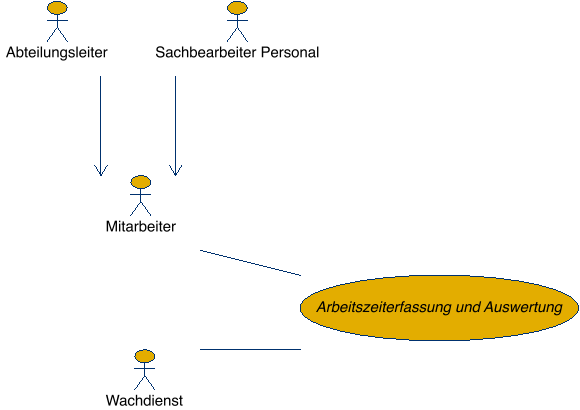
\includegraphics[width=0.9\linewidth]{UML/Export/Kontext.png}
	\caption{Kontextdiagramm zum SW-System \textit{Arbeitszeiterfassung und Auswertung}. Der Akteur Mitarbeiter generalisiert die Akteure Abteilungsleiter und Sachbearbeiter Personal}
	\label{Kontext}
\end{figure}

\chapter{Anwendungsfalldiagramme}
In einer weiteren Abstraktion werden die einzelnen Funktionen und ihre Kommunikationsbeziehungen zu den verschiedenen Akteuren dargestellt.

\section{AWD der groben Funktionalität}
Abbildung \ref{AWD} zeigt die oberste Abstraktionsebene der Anwendungsfalldiagramme. Die enthaltenen \textit{abstrakten Funktionen} Kapseln dabei mehrere verwandte Anwendungsfälle.

\vspace{1cm}
\begin{figure}[hbp]
	\centering
	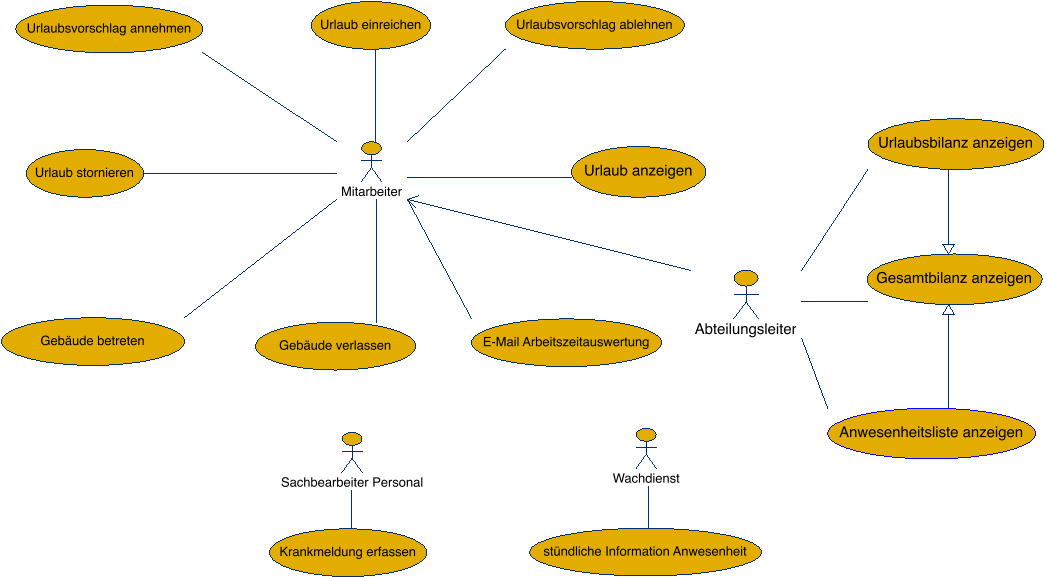
\includegraphics[width=\linewidth]{UML/Export/Grob.png}
	\caption{Anwendungsfalldiagramm zur groben übersicht.}
	\label{AWD}
\end{figure}

\newpage

\section{AWD der Funktionalität \textit{Urlaub planen}}
Beispielhaft wird nun die abstrakte Funktion \textit{Urlaub planen} näher betrachtet. Abbildung \ref{Urlaubplanen} zeigt das entsprechende AWD. Ein Mitarbeiter besitzt die Möglichkeiten Urlaub zu beantragen oder zu stornieren. Er kann weiterhin Urlaubsvorschläge seines Abteilungsleiters annehmen oder ebenfalls stornieren und seine persönlichen Urlaubsinformationen anzeigen.

\vspace{1cm}
\begin{figure}[hbp]
	\centering
	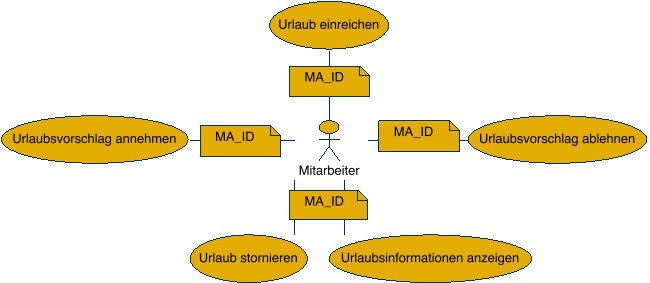
\includegraphics[width=\linewidth]{UML/Export/Urlaub_planen.png}
	\caption{Anwendungsfalldiagramm zur abstrakten Funktion \textit{Urlaub planen - Mitarbeiter}}
	\label{Urlaubplanen}
\end{figure}

\newpage

\section{Detaillierte Beschreibung der essentiellen Funktionalität \textit{Urlaub beantragen}}
Die essentielle Funktion \textit{Urlaub beantragen} gehört zu den kleinsten von anderen unabhängigen Anwendungsfällen. Beschreiben kann man sie wie folgt: \newline

Der Mitarbeiter verfasst seinen Urlaubsantrag, basierend auf seinen aktuellen Urlaubsinformationen. Der Antrag enthält die Daten MA-ID, Nachname, Vorname und eine Liste der zu beantragenden Urlaubstage. \newline

Nach \textsc{Chris Rupp} beschreibt man den Anwendungsfall alternativ unter Zuhilfenahme von Schatzschablonen folgenderma{\ss}en: \newline

SW-System \textit{Arbeitszeit erfassen und auswerten} muss dem Mitarbeiter die Möglichkeit bieten Urlaub einzureichen. \newline

Eine weitere Detaillierte Form der Modellierung bietet das Aktivitätsdiagramm. Es stellt die einzelnen Aktionen dar, die in einer Funktionalität gekapselt sind. Im Fall der essentiellen Funktionalität \textit{Urlaub beantragen} ist das Aktivitätsdiagramm trivial, dargestellt in Abbildung \ref{Aktivitaet}

\vspace{1cm}
\begin{figure}[hbp]
	\centering
	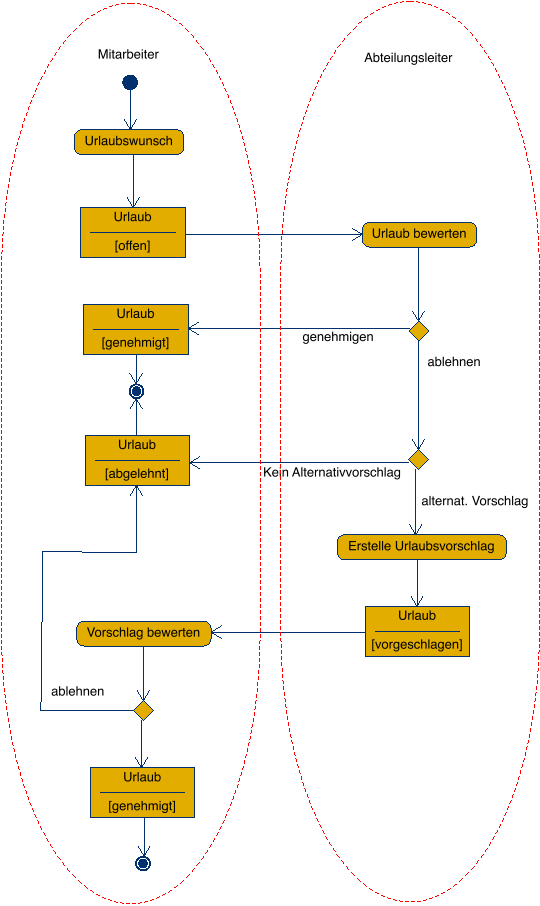
\includegraphics[width=\linewidth]{UML/Export/Urlaub_einreichen.png}
	\caption{Aktivitätsdiagramm der essentiellen Funktion \textit{Urlaub beantragen}.}
	\label{Aktivitaet}
\end{figure}

\chapter{Zustandsdiagramm eines Urlaubsantrages}
Der Anwendungsfall \textit{Urlaub planen} eines Mitarbeiters soll nun erneut detaillierter betrachtet werden. Dazu greifen wir das Objekt \textit{Urlaubsantrag} heraus und beschreiben es in einem Zustandsdiagramm genauer. Dieses Diagramm enthält die verschiedenen Zustände einer Betrachtungseinheit und beschreibt gleichzeitig die übergänge zwischen den Zuständen.

\vspace{1cm}
\begin{figure}[hbp]
	\centering
	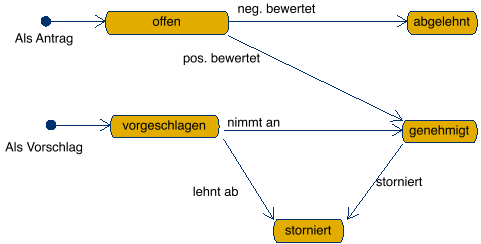
\includegraphics[width=0.9\linewidth]{UML/Export/Urlaubsantrag.png}
	\caption{Zustandsdiagramm des Objekts \textit{Urlaubsantrag}.}
	\label{Uantrag}
\end{figure}

\newpage

\chapter{Entity Relationship Model}

\begin{figure}[hbp]
	\centering
	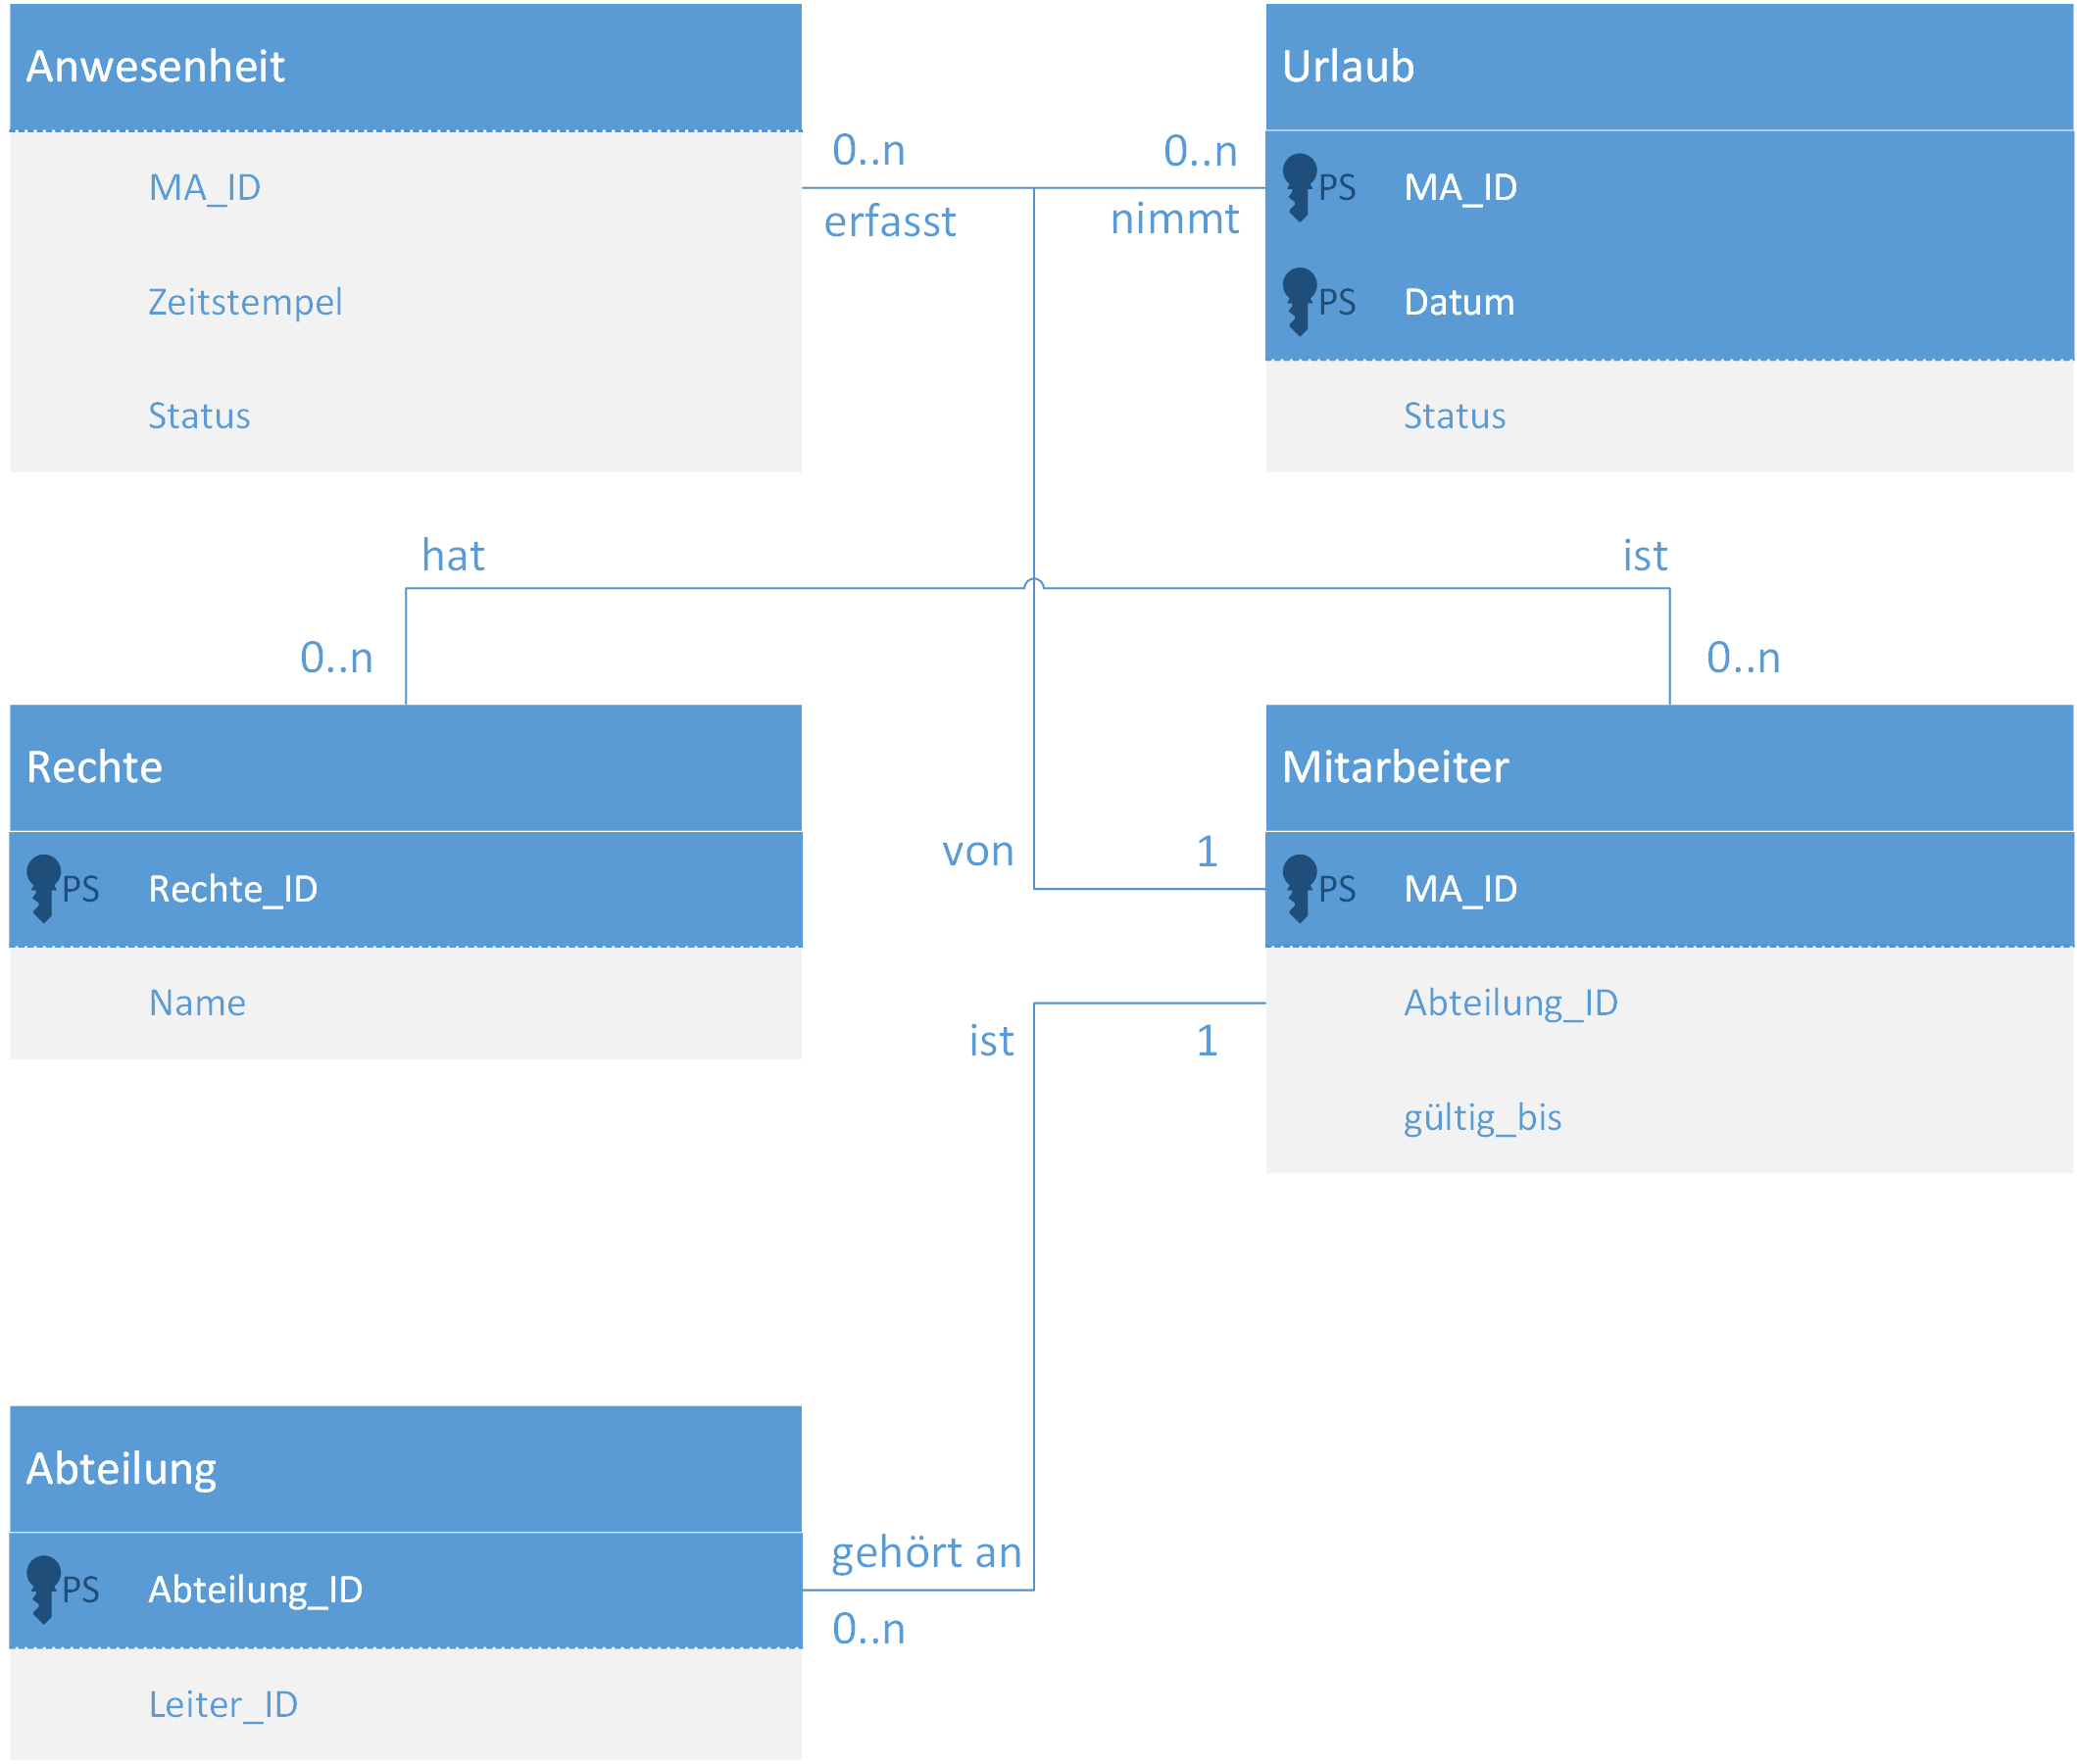
\includegraphics[width=1\linewidth]{UML/Export/erm.png}
	\caption{Entity Relationship Model aller essentiellen Funktionen}
	\label{ERM}
\end{figure}

\newpage
\paragraph*{Detaillierte Beschreibung des Entity Relationship Model}\mbox{} \\

Die Tabelle Mitarbeiter enthält alle \textit{Mitarbeiter}, indiziert unter dem Primär\-schlüssel \textit{MA\_ID}.
Außerdem gibt es ein Attribut \textit{gültig\_bis} um die Gültigkeit der Ausweise zu speichern.
Die Tabelle könnte weitere Informationen enthalten, wie z.B. \glqq Nachname\grqq, \glqq Vorname\grqq, oder \glqq Geburtsdatum\grqq. \newline

Jeder Mitarbeiter ist einer beliebigen Anzahl an Abteilungen zugehörig, weshalb eine Tabelle \textit{Abteilung} existiert.
Die Abteilungen der Firma sind unter dem Primärschlüssel \textit{Abteilung\_ID} indiziert.
Jede Abteilung besitzt einen Abteilungsleiter, der durch den Fremdschlüssel \textit{Leiter\_ID}, welcher sich auf eine \textit{MA\_ID} bezieht, beschrieben wird. \newline

Des Weiteren hat jeder Mitarbeiter eine beliebige Anzahl an Rechten, weshalb eine Tabelle \textit{Rechte} existiert.
In dieser sind diese unter dem Primärschlüssel \textit{Rechte\_ID} indiziert.
Jedem Eintrag wird ein \textit{Name} zugeordnet, um in der Software auf den jeweiligen Eintrag über den Namen zuzugreifen.
Dabei würde die Software z.B. die Verknüpfung von Rechte\_ID auf Name umkehren und lokal zwischenspeichern, weshalb Rechte\_ID als Primärschlüssel trotz allem sinnvoll ist. \newline

Die Anwesenheitserfassung wird durch die Tabelle \textit{Erfassung} ermöglicht.
Unter einem \textit{Zeitstempel} wird in Verknüpfung mit einem Mitarbeiter, welcher unter seiner \textit{MA\_ID} identifiziert wird, der \textit{Status} aufgezeichnet.
\textit{MA\_ID} würde sich hierbei als Fremdschlüssel auf einen Mitarbeiter beziehen.
\textit{Status} enthält die Art des Eintrages, sprich \glqq betreten\grqq oder \glqq verlassen\grqq.
Diese Tabelle enthält keinen Primärschlüssel, da eine MA\_ID zusammen mit dem Zeitstempel und notfalls dem Status zwar praktisch einen Primärschlüssel bilden würden, dies jedoch theoretisch nicht der Fall ist.
Dies Begründet sich damit, dass ein Primärschlüssel in dieser Tabelle keinen Nutzen hätte.
Des Weiteren sollte auch die theoretische Korrektheit gewährleistet werden.
Stattdessen sollte sich z.B. in einer relationalen Datenbank ein regulärer Index auf MA\_ID und auf dem Zeitstempel für die Auswertung als ausreichend erweisen. \newline

Zuletzt existiert die Tabelle \textit{Urlaub} um Urlaubsanträge zu erfassen.
Hier werden, unter einem \textit{Datum} und im Bezug auf einen Mitarbeiter mittels seiner \textit{MA\_ID}, Urlaubstage gespeichert.
Möchte der Mitarbeiter mehrere Tage Urlaub nehmen so müssen mehrere Einträge in der Tabelle erstellt werden.
Die Alternative ist es ein \glqq Startdatum\grqq und ein \glqq Enddatum\grqq des Urlaubs zu speichern.
Das hier vorgeschlagene Konzept ist jedoch der Alternative überlegen, da es zwar mehr Einträge benötigt, dies jedoch die Implementierung stark vereinfacht und etwaige Fehler verhindert.
Außerdem existiert ein Attribut \textit{Status}, welches den Status des Antrages enthält, sprich: \glqq offen\grqq, \glqq abgelehnt\grqq, oder \glqq genehmigt\grqq.

\newpage

\chapter{Glossar}
Der abschlie{\ss}ende Glossar soll es Personen aus verschiedenen Fachgebieten möglich machen, die vorliegende Anforderungsanalyse zu verstehen und mit ihr arbeiten zu können. Dazu werden wichtige Fachbegriffe aus dem Kontext des Software Engineering und der Anforderungsanalyse beschrieben.

\section{Allgemeiner Glossar}
\paragraph{Anwendungsfall}
Eine abstrakte Darstellung einer vom Software-System angebotenen Funktionalität (Aktivität). Er kapselt eine Menge von Aktionen, die sequentiell, bediengungsabhängig oder zyklisch abgearbeitet werden. Ein Anwendungsfall wird in Folge von Dateneingaben oder zeitlichen Ereignissen ausgelöst und führt in der Regel zu einem von au{\ss}en sichtbarem Ergebnis.

\paragraph{Anwendungsfalldiagramm}
Das Anwendungsfalldiagramm, kurz AWD, stellt die funktionalen Anforderungen (Aktivitäten) aus Sicht des Anwenders dar. Diese Aktivitäten werden zu den Beteiligten aus dem Kontext (Akteuren) in Beziehung gesetzt.

\paragraph{Akteur}
Ein Akteur ist die abstrakte Darstellung einer externen Instanz, die mit dem System kommuniziert.

\paragraph{Entity Relationship Model} Diagram zum allgemeinen abstrakten Entwurf der Datenstruktur.

\paragraph{Kontextdiagram} Veranschaulichung aller äußeren Wechselwirkungen mit dem gesamten Projekt.


\section{Projektbezogener Glossar}
\paragraph{Anwesenheit} Die Zeitspanne zwischen dem Ankommen des Mitarbeiters am Arbeitsplatz und seinem Verlassen dessen.

\paragraph{Arbeitstag} 8 Stunden

\paragraph{Arbeitswoche} 40 Stunden

\paragraph{Mitarbeiter-ID} Die eindeutige Kennung eines Mitarbeiters, hier eine 6-stellige alphanumerische Zeichenfolge

\paragraph{Zeitstempel} Ein Zeitpunkt formatiert nach ISO 8601, mindestens bis zur Sekunden-Auflösung.



%\begin{itemize}
%	\item abstrakte Funktion
%	\item essentielle Funktion
%	\item Entity Relationship Model
%	\item Unified Modeling Language
%	\item t.b.c
%\end{itemize}


\end{document}
